% SC3000 --- Chapter 1: Introduction to Intelligent Agents (0->100 ground-up)
\chapter{Introduction: Intelligent Agents}
\label{ch:intro}

\begin{quote}
\emph{``An agent is anything that can be viewed as perceiving its environment through sensors and acting upon that environment through actuators.''} --- Stuart Russell and Peter Norvig. This chapter builds that idea from everyday intuition to a precise engineering framework.
\end{quote}

\noindent\fbox{\parbox{\dimexpr\linewidth-2\fboxsep-2\fboxrule}{%
\textbf{From zero: no AI background assumed.} We start from what you already know---thermostats, phone apps, people---and build up \emph{agent}, \emph{rationality}, \emph{PEAS}, and a map of AI history before any search or learning algorithm. Every term is defined on first use, picture first, then formula.}}
\vspace{0.4em}

\section*{Learning Outcomes}
After this chapter you will be able to:
\begin{enumerate}[label=(L\arabic*)]
    \item define \emph{agent}, \emph{percept}, \emph{action}, and \emph{agent function} and map them to sensors and actuators;
    \item state the \emph{rational agent} criterion and distinguish rationality from omniscience and perfection;
    \item specify a task environment with the \emph{PEAS} framework (Performance, Environment, Actuators, Sensors);
    \item classify environments along PEAS dimensions (observable, deterministic, episodic, etc.);
    \item recount major milestones of AI history and why each shifted the field.
\end{enumerate}

% ============================================================
\section{What Is an Agent?}
\label{sec:what-is-agent}
\paragraph{Intuition.} Look at a room thermostat. It \emph{senses} temperature, compares it to a set-point, and \emph{acts} by switching the heater on or off. You do the same: eyes and ears sense, hands and voice act. The thermostat, a chatbot, a self-driving car, and you all fit one pattern---a loop with the world.

\paragraph{Formal definition.} An \emph{agent} perceives its \emph{environment} through \emph{sensors} and acts through \emph{actuators}. At time $t$ it receives a \emph{percept} $p_t$; the full history $p_1,\dots,p_t$ is the \emph{percept sequence}. The agent's behaviour is an \emph{agent function}
\[
f: \mathcal{P}^* \to \mathcal{A},\qquad f(p_1,\dots,p_t)=a_t,
\]
mapping every percept sequence to an action. The \emph{agent program} is the concrete implementation of $f$ on an architecture (hardware + software).

\paragraph{Example.} Vacuum world: two squares A and B, dirt appears at random. Percepts are $[\textit{location},\textit{dirt?}]\in\{A,B\}\times\{\textit{Dirty},\textit{Clean}\}$. Actions are $\{\textit{Left},\textit{Right},\textit{Suck},\textit{NoOp}\}$. The sequence $[A,\textit{Dirty}],[A,\textit{Clean}],[B,\textit{Dirty}]$ maps to $a_3=\textit{Suck}$ under a sensible $f$.

\begin{figure}[h]
\centering
\begin{tikzpicture}[
  agentbox/.style={draw=blue!60!black, thick, fill=blue!12, rounded corners=4pt, minimum width=3.2cm, minimum height=1.6cm, align=center},
  envbox/.style={draw=green!50!black, thick, fill=green!12, rounded corners=4pt, minimum width=3.2cm, minimum height=1.6cm, align=center},
  arrowP/.style={-{Latex[length=3mm]}, thick, color=orange!70!black},
  arrowA/.style={-{Latex[length=3mm]}, thick, color=violet!70!black}
]
% Agent
\node[agentbox] (agent) at (0,0) {\textbf{Agent}\\[2pt]\scriptsize sensors $\to$ agent function $f$ $\to$ actuators};
% Environment
\node[envbox] (env) at (7,0) {\textbf{Environment}\\[2pt]\scriptsize state $s_t$ evolves};
% Percepts arrow (environment -> agent, top)
\draw[arrowP] (env.north) -- ++(0,0.9) -- ++(-7,0) -- (agent.north)
  node[midway, above, font=\scriptsize, fill=orange!10, rounded corners=2pt, inner sep=2pt] {percepts $p_t$};
% Actions arrow (agent -> environment, bottom)
\draw[arrowA] (agent.south) -- ++(0,-0.9) -- ++(7,0) -- (env.south)
  node[midway, below, font=\scriptsize, fill=violet!10, rounded corners=2pt, inner sep=2pt] {actions $a_t$};
% Sensors / actuators labels
\node[font=\tiny, fill=white, inner sep=1pt] at (1.1,0.55) {sensors};
\node[font=\tiny, fill=white, inner sep=1pt] at (1.1,-0.55) {actuators};
% Legend
\node[font=\tiny, align=left, fill=yellow!8, draw=gray!40, rounded corners=2pt, inner sep=3pt] at (3.5,-2.0) {\textcolor{orange!70!black}{$\blacksquare$ percepts (sense)} \quad \textcolor{violet!70!black}{$\blacksquare$ actions (act)}};
\end{tikzpicture}
\caption{Agent--environment loop. The agent receives percepts through sensors, selects $a_t=f(p_1,\dots,p_t)$, and modifies the environment through actuators; the environment updates to $s_{t+1}$ and emits the next percept.}
\label{fig:agent-loop}
\end{figure}

% ============================================================
\section{Rationality and Performance}
\label{sec:rationality}
\paragraph{Intuition.} A good thermostat is not one that \emph{knows} the weather tomorrow; it is one that does the \emph{best it can} with the sensor it has and the energy bill you care about. Rationality is about expected outcome, not psychic perfection.

\paragraph{Formal criterion.} Fix a \emph{performance measure} $U$ that scores environment histories (e.g., $+10$ per clean square, $-1$ per move). A \emph{rational agent} acts to maximise \emph{expected} $U$ given the percept sequence, its built-in knowledge, and the actions it can execute:
\[
a_t^* = \arg\max_{a\in\mathcal{A}} \mathbb{E}\,[U \mid p_{1:t},\, \text{knowledge},\, a].
\]
Rational $\neq$ omniscient (which knows the true outcome) and $\neq$ clairvoyant (which knows all future percepts). Rationality also requires \emph{autonomy}: the agent should learn from experience rather than rely solely on designer priors.

\paragraph{Example.} Crossing a road: performance is safety $+$ speed. An omniscient agent would know no car comes and stride blindly; a rational agent looks both ways, waits for evidence, and then crosses---even though looking costs a second. If it never learns that a certain crossing is usually empty, it lacks autonomy.

% ============================================================
\section{Specifying Tasks: The PEAS Framework}
\label{sec:peas}
\paragraph{Intuition.} ``Build me an AI for hospitals'' is not a specification. Four questions make it one: How will we \emph{measure} success? What \emph{world} will it face? What can it \emph{do}? What can it \emph{see}?

\paragraph{Formal framework.} Every task environment is described by \textbf{PEAS}:
\begin{description}[leftmargin=1.2em, itemsep=0.3em]
    \item[P --- Performance measure] The objective criterion $U$ the rational agent maximises.
    \item[E --- Environment] The world, other agents, and dynamics the agent interacts with.
    \item[A --- Actuators] The actions/channels available to the agent.
    \item[S --- Sensors] The percepts/inputs through which the agent observes.
\end{description}
Table~\ref{tab:peas} fills PEAS for four representative agents. Designing PEAS \emph{before} choosing an algorithm forces clarity about the trade-off you actually care about.

\begin{table}[h]
\centering
\resizebox{\linewidth}{!}{%
\begin{tabular}{lllll}
\toprule
\textbf{Agent} & \textbf{Performance} & \textbf{Environment} & \textbf{Actuators} & \textbf{Sensors} \\
\midrule
Self-driving taxi & Safety, time, comfort, profit & Roads, traffic, passengers & Steering, brake, display & Cameras, lidar, GPS, mic \\
Medical diagnosis & Accuracy, cost, explanation & Patient, hospital, diseases & Screen, report, referral & Symptoms, labs, images \\
Part-picking robot & \% parts correctly binned & Conveyor, bins, other arms & Arm, gripper, sorter & Camera, force sensor \\
Chatbot tutor & Learning gain, satisfaction & Student, curriculum, network & Text, speech, exercises & Keystrokes, answers, clicks \\
\bottomrule
\end{tabular}}%
\caption{PEAS descriptions make the design problem explicit. Changing any column (e.g., adding a sensor) changes the rational policy.}
\label{tab:peas}
\end{table}

Environments are also characterised along six dimensions: fully vs.\ partially \emph{observable}, single vs.\ multi \emph{agent}, \emph{deterministic} vs.\ stochastic, \emph{episodic} vs.\ sequential, \emph{static} vs.\ dynamic, \emph{discrete} vs.\ continuous. A taxi is partially observable, multi-agent, stochastic, sequential, dynamic, continuous; a crossword puzzle is fully observable, single-agent, deterministic, sequential, static, discrete.

\begin{lstlisting}[language=Python, caption={PEAS as a data structure: specifying a task before coding the agent.}, label={lst:peas}]
from dataclasses import dataclass

@dataclass
class PEAS:
    performance: str
    environment: str
    actuators: list
    sensors: list

taxi = PEAS(
    performance="minimise time + maximise safety + profit",
    environment="roads, traffic, pedestrians, weather",
    actuators=["steer", "accelerate", "brake", "horn", "display"],
    sensors=["camera", "lidar", "GPS", "microphone", "odometer"]
)

def is_rational(action, percept_seq, peas: PEAS) -> bool:
    """Stub: compare action against expected performance measure."""
    # In Ch.2-5 this becomes search; in Ch.8 it becomes learning.
    return True  # placeholder for expected-utility test
\end{lstlisting}

% ============================================================
\section{A Brief History of AI}
\label{sec:history}
\paragraph{Intuition.} AI did not appear with ChatGPT. It is an 80-year arc of big claims, winters, and quiet engineering that suddenly looked like magic when scale and data caught up.

\paragraph{Timeline (formal milestones).} Five eras are conventional: \emph{foundations} (1943--1955), \emph{symbolic AI} (1956--1974), \emph{knowledge and expert systems} (1969--1986), \emph{statistical learning} (1986--2011), \emph{deep learning and foundation models} (2012--present).

\begin{figure}[h]
\centering
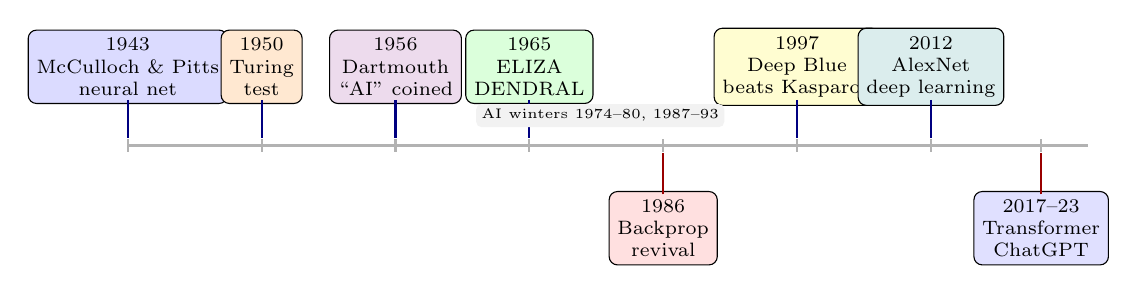
\begin{tikzpicture}[every node/.style={font=\scriptsize}]
% timeline line
\draw[thick, gray!60] (0,0) -- (12.2,0);
\foreach \x in {0,1.7,3.4,5.1,6.8,8.5,10.2,11.6} \draw[thick, gray!60] (\x,0.08)--(\x,-0.08);
% nodes
\node[draw, fill=blue!14, rounded corners=3pt, align=center, inner sep=3pt] at (0,1.0) {1943\\McCulloch \& Pitts\\neural net};
\node[draw, fill=orange!18, rounded corners=3pt, align=center, inner sep=3pt] at (1.7,1.0) {1950\\Turing\\test};
\node[draw, fill=violet!14, rounded corners=3pt, align=center, inner sep=3pt] at (3.4,1.0) {1956\\Dartmouth\\``AI'' coined};
\node[draw, fill=green!14, rounded corners=3pt, align=center, inner sep=3pt] at (5.1,1.0) {1965\\ELIZA\\DENDRAL};
\node[draw, fill=red!12, rounded corners=3pt, align=center, inner sep=3pt] at (6.8,-1.05) {1986\\Backprop\\revival};
\node[draw, fill=yellow!18, rounded corners=3pt, align=center, inner sep=3pt] at (8.5,1.0) {1997\\Deep Blue\\beats Kasparov};
\node[draw, fill=teal!14, rounded corners=3pt, align=center, inner sep=3pt] at (10.2,1.0) {2012\\AlexNet\\deep learning};
\node[draw, fill=blue!12, rounded corners=3pt, align=center, inner sep=3pt] at (11.6,-1.05) {2017--23\\Transformer\\ChatGPT};
% arrows to line
\foreach \x in {0,1.7,3.4,5.1,8.5,10.2} \draw[thick, blue!50!black] (\x,0.58)--(\x,0.10);
\foreach \x in {6.8,11.6} \draw[thick, red!60!black] (\x,-0.62)--(\x,-0.10);
% winter label
\node[font=\tiny, fill=gray!10, rounded corners=2pt, inner sep=2pt] at (6.0,0.38) {AI winters 1974--80, 1987--93};
\end{tikzpicture}
\caption{Condensed history of AI. Colour groups eras: blue/orange = foundations, violet/green = symbolic, red/yellow = knowledge and competition, teal/blue = deep learning era. Winters mark funding contractions after over-promising.}
\label{fig:ai-timeline}
\end{figure}

Why it matters: each era changed what an agent could be. Logic gave us provably correct agents but brittle ones; expert systems added human knowledge but were costly to maintain; statistical learning let agents handle uncertainty; deep networks let them learn their own features from raw sensors.

% Simple reflex agent
\begin{lstlisting}[language=Python, caption={A simple reflex agent for the vacuum world. No memory beyond the current percept.}, label={lst:reflex}]
def simple_reflex_vacuum(percept):
    """percept = (location, status) where status in {'Dirty','Clean'}.
       Returns an action in {'Suck','Right','Left','NoOp'}."""
    location, status = percept
    if status == 'Dirty':
        return 'Suck'
    # otherwise move toward the other square
    if location == 'A':
        return 'Right'
    else:
        return 'Left'

# Simulation stub: percept sequence -> action
trace = [('A','Dirty'), ('A','Clean'), ('B','Dirty')]
for p in trace:
    print(p, "->", simple_reflex_vacuum(p))
\end{lstlisting}
Reflex agents work when the current percept suffices (fully observable, episodic). When history matters, we need model-based, goal-based, or utility-based agents---the subject of later chapters.

% ============================================================
\section{Chapter Notes}
Further reading: Russell \& Norvig Ch.~1--2 for the canonical PEAS and agent taxonomy; Nilsson (1998) for the historical arc; Turing (1950) for the imitation game. The PEAS table pattern is due to Russell \& Norvig and is the standard scoping tool in NTU SC3000 design exercises.

% ============================================================
\section{Exercises}
\label{sec:ch01-exercises}
\begin{enumerate}[label=E1.\arabic*, leftmargin=*, itemsep=0.7em]
    \item \textbf{Agent function vs.\ program.} Give the agent function $f$ for a 2-state thermostat (percepts $\{\textit{Cold},\textit{Hot}\}$, actions $\{\textit{On},\textit{Off}\}$) that turns heat on when cold and off when hot. Write the program as a Python dictionary lookup. Why can two different programs implement the same function?
    \item \textbf{Rationality, not omniscience.} A vacuum agent is penalised $-1$ per move and $+10$ per clean. It does not know whether dirt will reappear. Compare a rational agent that maximises expected score against an ``omniscient'' agent that knows the future dirt schedule. Give a percept sequence where they choose differently and compute expected vs.\ actual scores.
    \item \textbf{PEAS design.} Specify PEAS for (a) an AI tutor for SC2001 algorithms and (b) an automated warehouse picker. Fill one row of Table~\ref{tab:peas} for each. For each, state whether the environment is fully/partially observable, deterministic/stochastic, and episodic/sequential, and justify in one sentence per dimension.
    \item \textbf{Reflex limits.} Show that no simple reflex agent (mapping current percept only) can be rational in a partially observable vacuum world where the agent cannot sense its location (percept is only $\textit{Dirty}/\textit{Clean}$). Propose a minimal memory extension that restores rationality and sketch its code.
    \item \textbf{History and winters.} Pick two milestones from Fig.~\ref{fig:ai-timeline} (one before 1980, one after 2010). For each, name the bottleneck it removed and one new limitation it introduced that led to the next winter or shift.
\end{enumerate}
% End of Chapter 1
